\section{Meta Optimization Approach}

After the FMO step is developed and encapsulated, one may simply modify the weights used for the FMO iteratively, until a condition is met, or for a given number of steps.
We will therefore have one inner optimization (the FMO), and one outer optimization.
\begin{center}
	\begin{minipage}{.55\linewidth}
		\begin{algorithm}[H]
			\caption{Meta Optimization Algorithm Outline}
			\label{alg:meta_optim}
			\begin{algorithmic}
				\State initialize $w$
				\Repeat
					\State initialize $b$ \Comment{FMO starts}
					\Repeat
							\State \textcolor{Prune}{ $d = Lb$ \Comment{differentiable} }
							\State \textcolor{Prune}{ $c = \mathcal{C}(w, d)$ \Comment{differentiable} }
							\State \textcolor{Prune}{ back-propagate $c$ }
							\State \textcolor{Prune}{ update $b$ }
						\Until{\textit{FMO \textbf{stop condition}}} \Comment{FMO ends}
					\State update $w$
				\Until{\textit{Meta-optimization \textbf{stop condition}}}
			\end{algorithmic}
		\end{algorithm}
	\end{minipage}
\end{center}
The outer optimization step is not differentiable (or at least, not in a reasonable computation time).
Hence, we will be looking at gradient-free optimization methods.

\subsection{Expert Weight Adjustment}
Expert systems are computer systems emulating the decision-making of a human expert.

\paragraph{Simple Weight Increase}
One approach is to increase the weight of all constraints that are not met after each FMO optimization.
\begin{itemize}
	\item \textbf{Advantages:} Very simple to implement, and understand.
	\item \textbf{Disadvantages:} If none of the constraints is met, then the outer loop is stuck.
	This method might struggle to converge in complex cases where multiple constraints compete.
\end{itemize}

\paragraph{Inverse Proportional Weight Increase}
Another approach is to increase the weight of each constraint inversely proportional to how close it is to being met, quantifying the degree to which a constraint is satisfied.

Quantification Example: use the area bounded by the DVH constraint, and the DVH curve.
When this is zero, then the constraint is met.
\begin{itemize}
	\item \textbf{Advantages:} Still relatively easy to implement, and allows for a more nuanced adjustment of weights based on constraint satisfaction.
	\item \textbf{Disadvantages:} This method can lead to an oscillation phenomenon, where constraints fluctuate between satisfaction and violation.
\end{itemize}
Of course, 	one could add momentum to smooth the process, to fix the oscillation problem.
However, expert systems like these often require constant refinement, hence, this path is not viable for a credible clinical application.

% Full paper:
% https://github.com/pauldubois98/AIME2024/blob/main/llncs_formatting.pdf
\section{Radiotherapy Dose Optimization via Clinical Knowledge Based Reinforcement Learning (AIME 2024)}
\paragraph{Abstract}
%% Achieving optimal dose distribution in radiation therapy planning is a complex task, with contradicting goals. Yet, this step is crucial with profound implications for patient treatment.
%% The absence of universally agreed-upon constraints prioritization in radiation therapy planning complicates the definition of an optimal plan, requiring a delicate balance between multiple objectives. This balance usually ends up being done manually.
%A radiation therapy plan finds an equilibrium between goals with no universal prioritization. The delicate balance between multiple objectives is typically done manually.
%The optimization process is further hindered by complex mathematical aspects, involving non-convex multi-objective inverse problems with a vast solution space.
%Expert bias introduces variability in clinical practice, as the preferences of radiation oncologists and medical physicists shape treatment planning.
%
%To surmount these challenges, we propose a first step towards a fully automated approach, using an innovative deep-learning framework.
%Using a clinically meaningful distance between doses, we trained a reinforcement learning agent to mimic a set of plans.
%This method allows automatic navigation toward acceptable solutions via the exploitation of optimal dose distributions found by human planners on previously treated patients.
%As this is ongoing research, we generated synthetic phantom patients and associated realistic clinical doses.
%Our deep learning agent successfully learned correct actions leading to treatment plans similar to past cases ones.
%The incapacity to reproduce human-like dose plans hinders adopting a fully automated treatment planning system; this method could start paving the way towards human-less treatment planning system technologies. % "tie conclusion of reasoning why we do this technique."
%In future work, we hope to be able to apply this technique to real cases.

\subsection{Introduction}
%In contemporary radiation therapy, photon intensity modulated radiation therapy (IMRT) is a pivotal technique to attain precise and conformal dose distributions within target volumes \cite{xu_comparison_2017}.
%This achievement owes its realization to the advent of the multileaf collimator (MLC) \cite{galvin_characterization_1993}.
%Radiation therapy is now a reliable treatment for oncology \cite{valentini_survival_2009}.
%Despite this consensus, the way to deliver radiotherapy for its best result remains very dependent upon doctors.
%Moreover, there appears to be a large variability across physicians and centres, but in terms of 3D structures contouring and irradiation, constrains priorities \cite{variability_2021}.
%
%To achieve the best treatment, doctors must solve a complex inverse mathematical optimization problem with multiple trade-offs \cite{oelfke_inverse_2001} \cite{webb_physical_2003}.
%However, a lack of standardized prioritization of constraints makes the optimization a real challenge.
%The standard procedure nowadays is to guide computer optimization manually: dosimetrists manually update the settings of an optimizing software so-called Treatment Planning System (TPS) \cite{planification_website}.
%
%There have been many tries to create a metric that quantifies the quality of a treatment plan, such as Normal Tissue Complication Probabilities (NTCP), target coverage, conformity index, and heterogeneity index, among others/to name a few \cite{lyman_normal_1992} \cite{li_input_2022}\label{metrics}.
%However, they have yet to satisfy all radio-oncologists, and the only reliable way to assess a doctor's plan is to evaluate the dose-volume histograms (DVHs) themselves.
%
%As a result, Pareto surface exploration is unsuitable due to the lack of impartial quantitative measurement for a particular plan \cite{huang_pareto_2021}.
%Other meta-optimization techniques are similarly bounded for the same reason \cite{wu_optimization_2001} \cite{xing_optimization_1999}.
%An extra challenge to attend for those is the fact that not all cases have the same difficulty.
%Hence, for an "easy" case, doctors will require an excellent dose (in terms of the metrics mentioned above), while they can be more permissive for "harder" cases.
%The context-aware acceptability criteria make the acceptability of a plan hard to define in general.
%
%Reinforcement learning (RL) is a machine learning paradigm that trains agents to make sequential decisions in dynamic environments \cite{brooks_what_2021}.
%Agents learn to optimize their actions to achieve long-term objectives through trial and error guided by rewards or penalties.
%The decisions taken by dosimetrists when optimizing treatment can be formalized as an RL problem.
%Moreover, dosimetrists can guide the TPS towards an acceptable plan but usually struggle to explain their decision while interacting with the TPS.
%The difficulty in explaining why certain decisions are taken suggests using deep RL over expert-based methods.
%This setup is similar to image recognition, where one can say a picture represents a car or a boat but struggles to explain why.
%
%The study’s primary hypothesis is that all the information needed to decide what weights should be changed in the objective function used by the optimizer relies on the Dose Volume Histograms (DVHs).
%Our hypothesis is supported by the fact that dosimetrists almost solely use DVHs plots.
%In order to learn the actions of dosimetrists who use a TPS to optimize doses, we leverage deep learning.
%This is done by training an agent that takes the DVHs as the input of the current optimized dose, and predicts the evaluation of possible weights changes.
%
%Typically, access to the exact actions taken by human dosimetrists on the TPS is unavailable (as clinics do not usually store this data; only the final plan is held).
%Therefore, we only use the dose distributions of previously treated patients to train our model.
%This partial availability of data suggests the use of RL.

\subsection{Materials and Methods}
%We introduce a new paradigm for reward-based dosimetrist RL agents.
%This new reward system aims to improve how human-optimized doses are mimicked.

\subsubsection{Reinforcement Learning Reward}

%\begin{figure*}
%	\centering
%	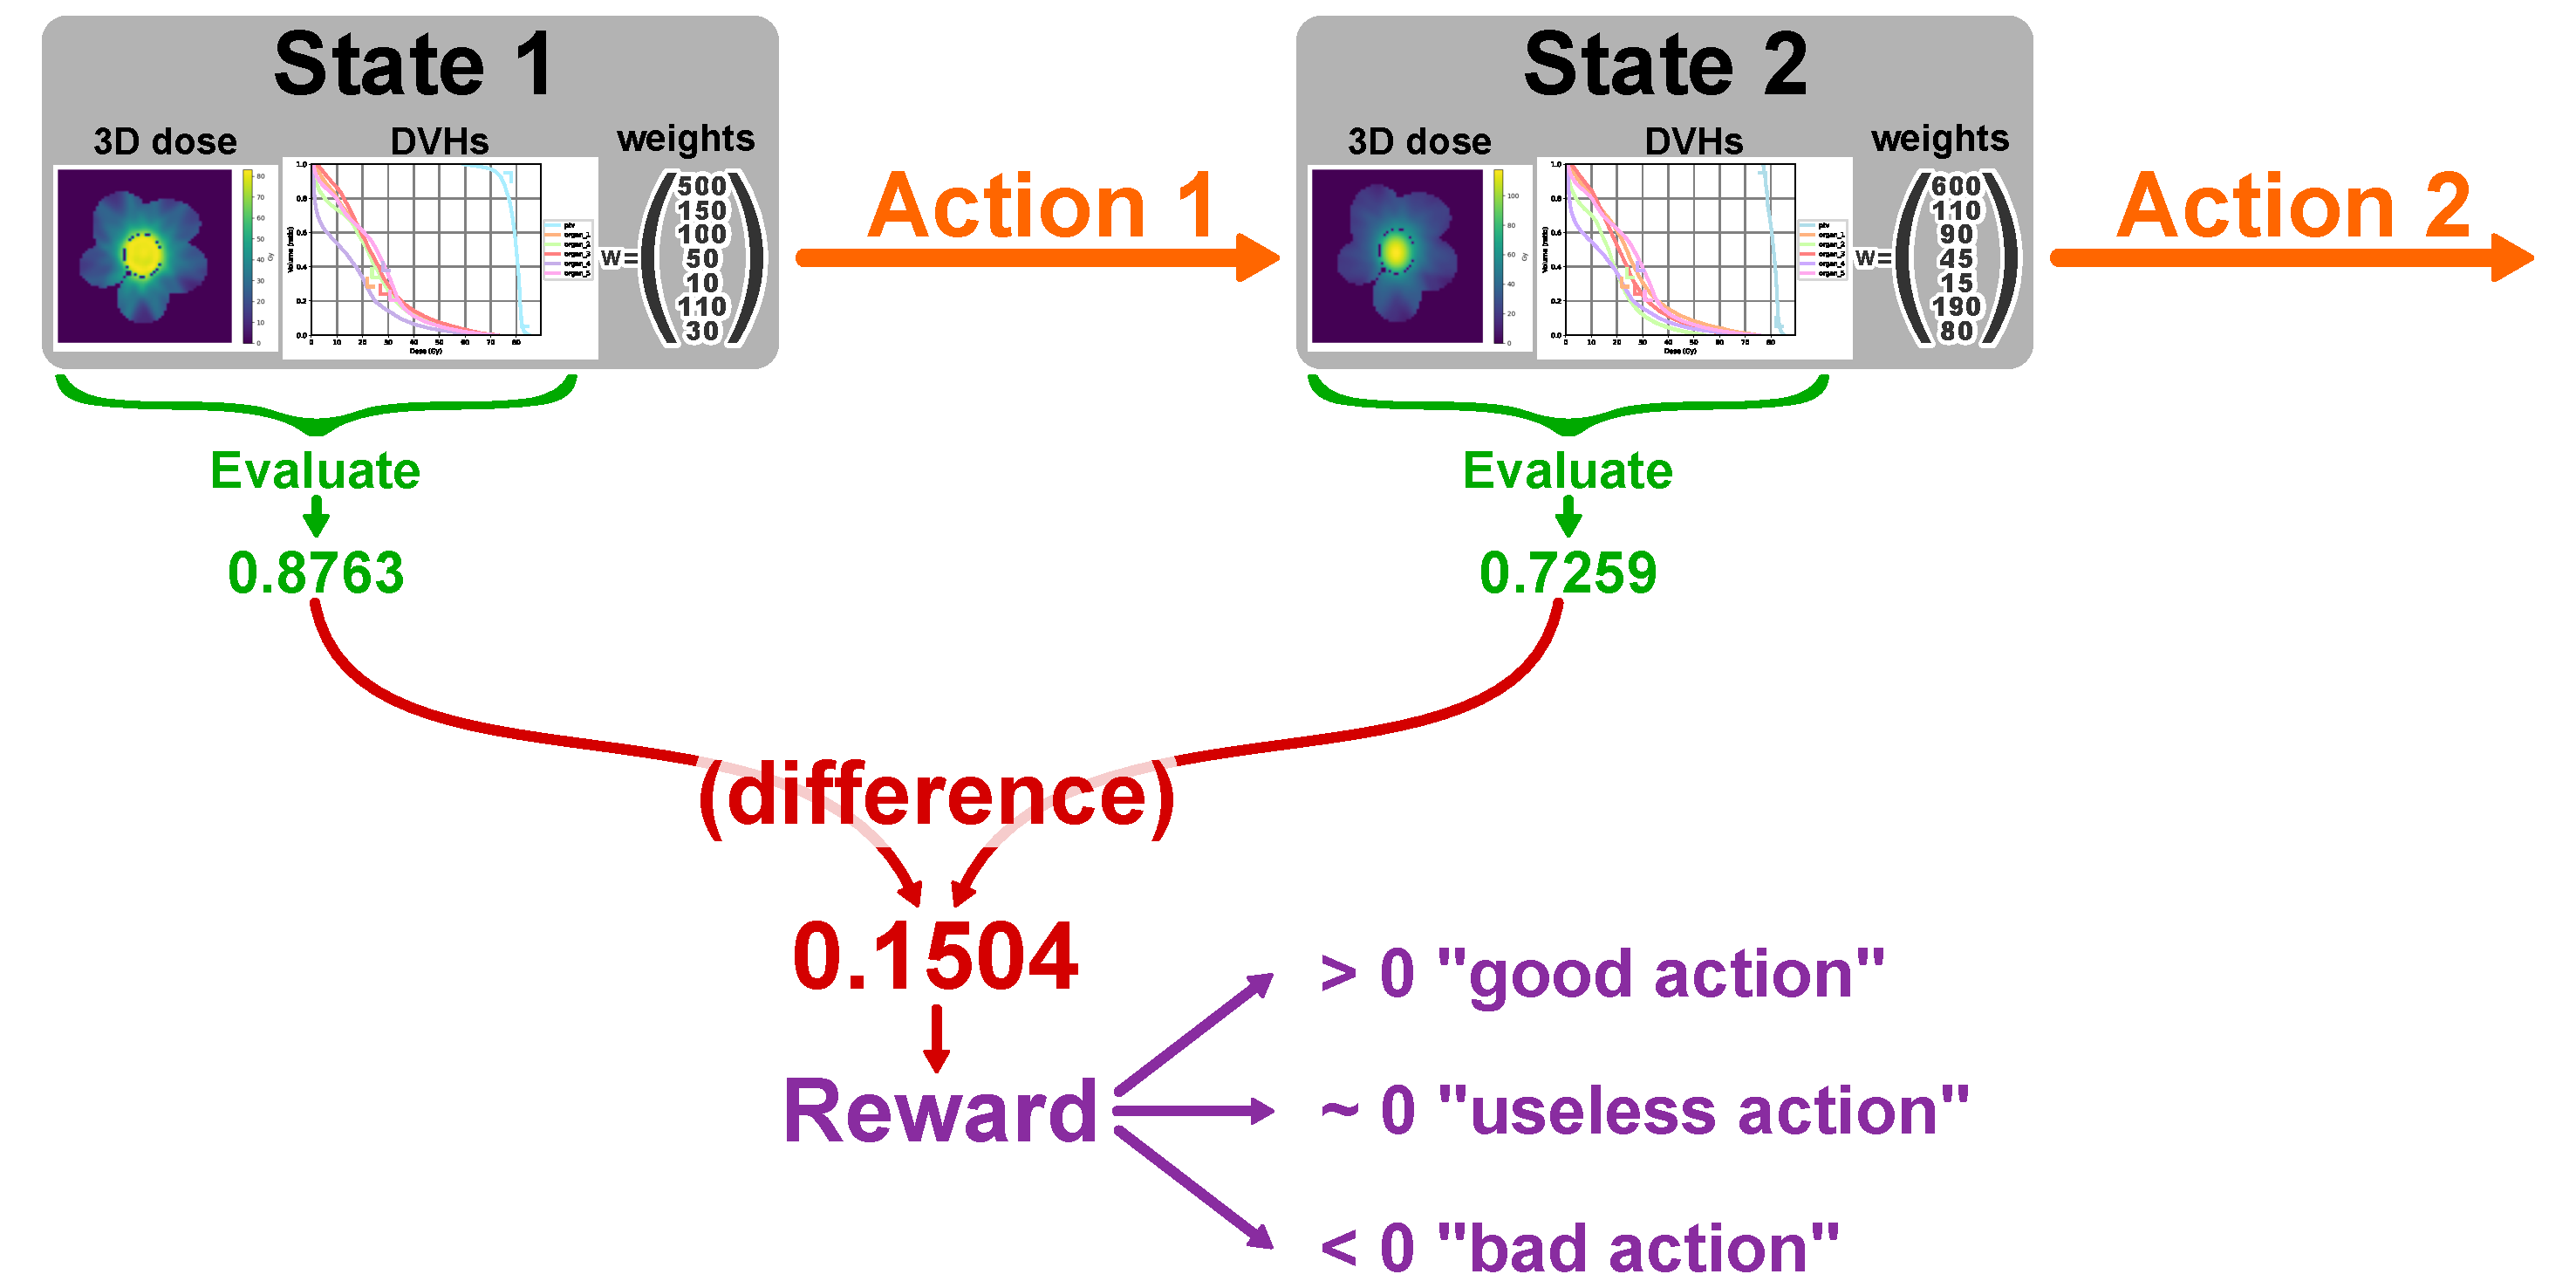
\includegraphics[width=0.9\textwidth]{AIME/reward.pdf}
%	\caption{Classical reinforcement learning reward for automatic dosimetry.}
%	\label{fig:reward_fig}
%\end{figure*}
%
%In classical RL, we want $V(S_t) = R_t + \gamma V(S_{t+1})$
%(so the update is $V(S_t) \leftarrow (1-\alpha) V(S_t) + \alpha \left[ R_{t+1} + \gamma V(S_{t+1}) \right]$).
%In the context of dose optimization, the reward $R_t$ is defined as $R_t = \mathcal{E}(S_{t+1}) - \mathcal{E}(S_t)$, where $\mathcal{E}$ is a function that evaluates the quality of a state (such that higher is better; if lower is better, then swap $s_t$ and $S_{t+1}$).
%
%The evaluation $\mathcal{E}$ can be one or a mixture of the metrics mentioned in the introduction (Section \ref{metrics}) \cite{shen_hierarchical_2021} \cite{shen_intelligent_2019} \cite{moreau_reinforcement_2021}.
%This setup may leverage knowledge about which actions to perform instead of guessing randomly, as a meta-optimizer would do.
%This could potentially gain some computation time.
%
%However, this technique does not use past plans; it only needs the optimizer inputs (CT, structures contours).
%We propose using the availability of past treatment plans to more accurately reflect the complexity of decisions made by dosimetrists and better match their expectations of a fully automatic treatment planning system.
%
%As developed in previous work, we can derive a distance between dose plans \cite{paul_dubois_novel_2024}.
%If we consider the clinical dose of past cases (used for training) as the best achievable one, we can evaluate a dose plan by computing its distance from the clinical dose plan.
%
%Let $D_t$ be the dose associated with $S_t$, and $D_C$ the clinical dose.
%We then define $\mathcal{E}(S_t) = \mathcal{D}(D_t, D_C)$.
%Since, in that case, $\mathcal{E}(S_t)$ should be minimized, we will define the reward as $$R_t = \mathcal{E}(S_t) - \mathcal{E}(S_{t+1}) = \mathcal{D}(D_t, D_C) - \mathcal{D}(D_{t+1}, D_C).$$
%This reward can be interpreted as the "distance gained to the clinical dose". 

\subsubsection{Architecture}
%We use a dense neural network, which inputs the DVHs and current normalized weight values.
%It outputs the $Q(s, a)$ value for each possible action $a$.
%Dense layers are very prone to overfitting.
%In order to force the network to actually predict the following evaluation for each possible action, without overfitting, we incorporated a bottleneck in the network (Figure \ref{fig:architecture}).
%Compressing the information stops the network from overfitting.
%Networks with such architecture show very little difference between training and validation sets (see Figure \ref{fig:losses_training}).
%
%\begin{figure*}
%	\centering
%	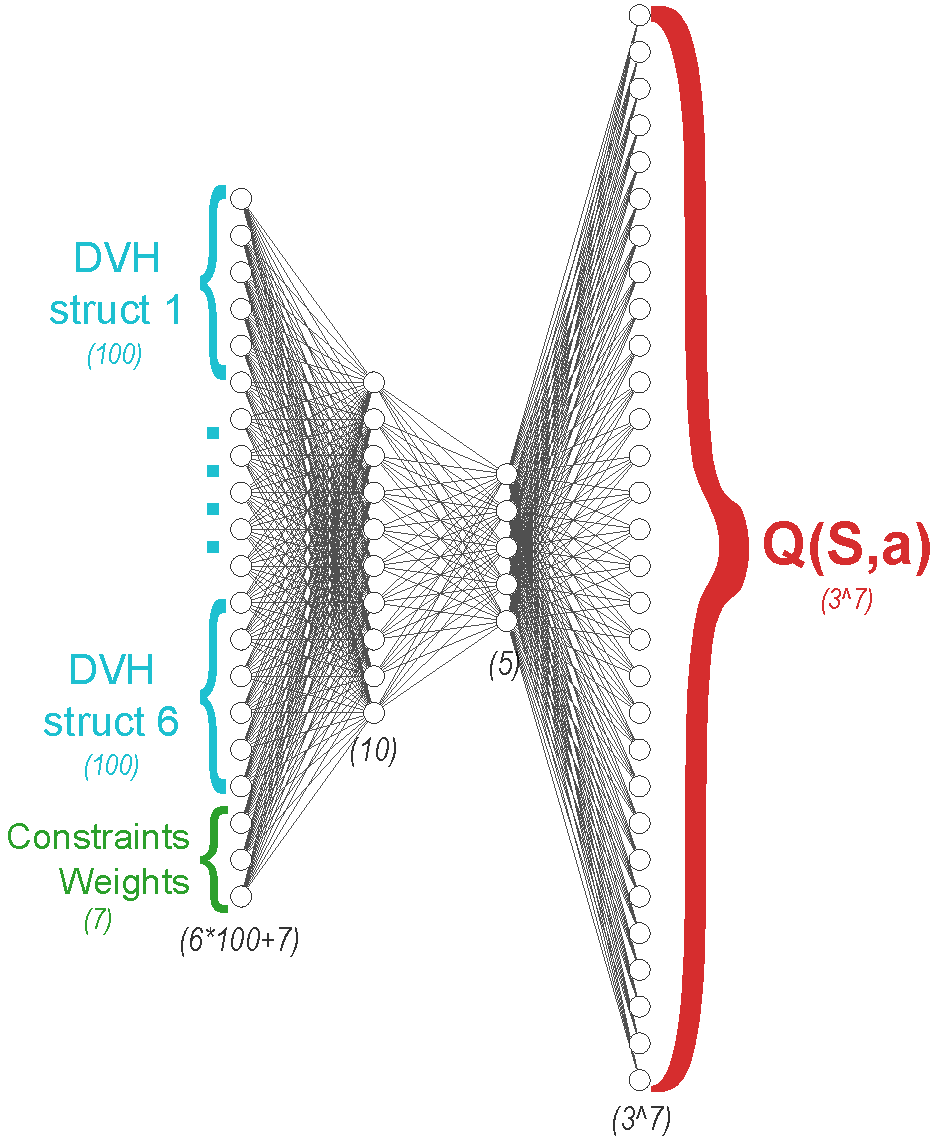
\includegraphics[width=5cm]{AIME/architecture_all_actions.pdf}
%	\hspace{0.5cm}
%	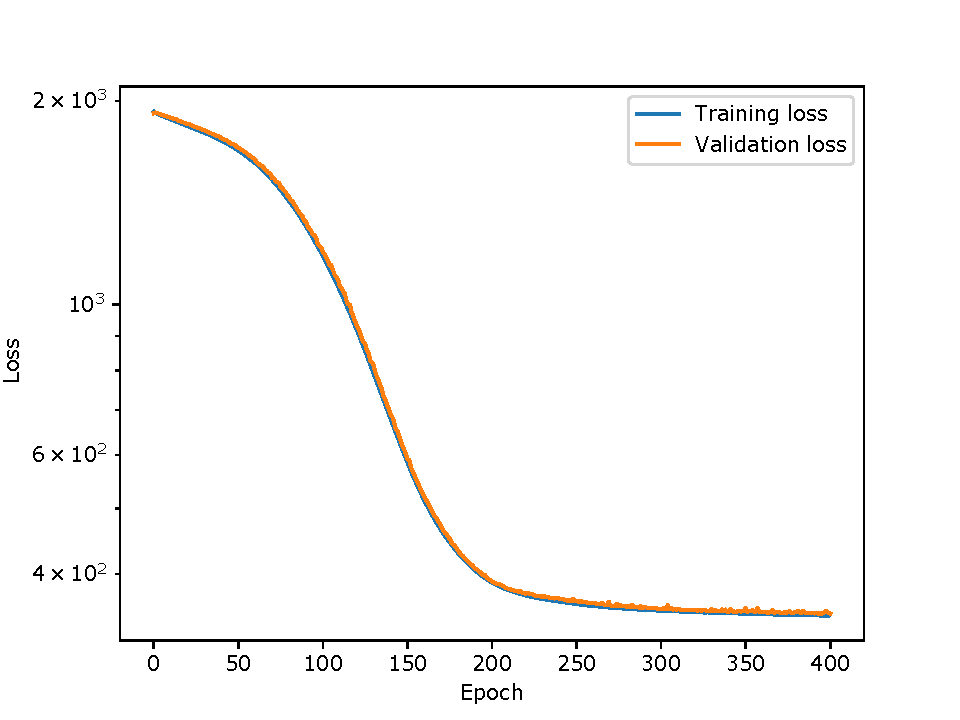
\includegraphics[width=6cm]{AIME/losses-distance.pdf}
%	\caption{Neural network architecture and loss evolution while training.}
%	\label{fig:architecture}
%	\label{fig:losses_training}
%\end{figure*}

\subsubsection{Avoiding Off-Distribution}
%We generated a training set of over 125k actions (this took five days on an NVIDIA GeForce GTX 1080).
%Despite this relatively large dataset, we have not explored exhaustively the state-actions space, and the network still lands off-distribution.
%This can easily be spotted when the predicted $Q$ value is greater than the current distance to the clinical dose; we choose to ignore those predictions, and in fact all outlier predictions.
%The justification is that our set of actions is limited, no action will suddenly drastically improve the plan.
%It is the combination of several sequential actions that allows good plan optimization.
%Therefore, while testing, we choose the action with the best prediction, while passing the outlier test just mentioned.
%
%\subsection{Results}
%Figure \ref{fig:distance} shows how the distance between our RL agents performs over five steps on 30 test patients (unseen during the training).
%A lower distance is interpreted as an improved dose, since it is closer to the best dose, which is the clinical one.
%\begin{figure*}
%	\centering
%	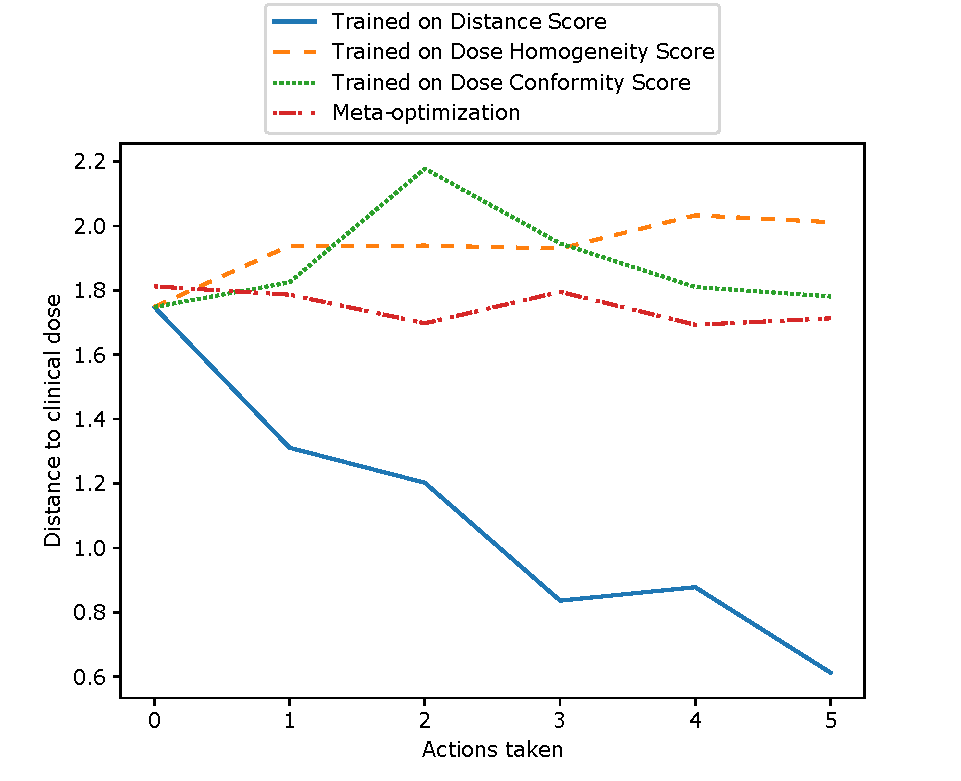
\includegraphics[width=0.6\textwidth]{AIME/DistanceToClinicalDose.pdf}
%	\caption{Average distance between RL agent's dose and clinical dose.}
%	\label{fig:distance}
%\end{figure*}


\subsubsection{Quantitative Results}
%The network converged on the training data, and validation showed minor overfitting.
%For testing, we generated 30 brand new cases that we again manually optimized.
%We then used the RL model to perform the optimization of these 30 unseen cases.
%On average, our model was able to reduce the dose distance with manually optimized dose by a factor of $~3$ (from $~1.8$ at iteration $0$ to $~0.6$ at iteration $4$), as shown in Table \ref{table:results}.
%
%We remark from the Table \ref{table:results} that the homogeneity score and conformity score give similar results.
%Classical meta-optimization performs well, but needs a metric to elect the best dose (during the test, the clinical dose is unknown, so the DVHs distance metric is not available).
%We also observe that clinical doses are not always scoring high (in this test set, a high conformity, but low homogeneity compared to automatic techniques).
%This show the difficulty to create a metric that capture all the complexity of a clinically acceptable dose.
%
%\begin{table}
%	\begin{center}
%		\begin{tabular}{| c || c | c | c |} 
%			\hline
%			Agent $\backslash$ Metric & Mean Final Distance$^*$ & Homogeneity Score$^\dagger$ & Conformity Score$^\dagger$ \\ 
%			\hline
%			RL Distance Score & \textbf{0.612} & 1.871 & 0.406 \\ 
%			RL Homogeneity Score & 2.012 & \textbf{4.387} & 0.567 \\
%			RL Conformity Score &  1.770  & 4.017 & 0.507 \\
%			Meta-optimization & N/A & 4.117 & \textbf{0.610} \\
%			\textit{Clinical doses} & \textit{0} & \textit{1.541} & \textit{0.580} \\	
%			\hline
%		\end{tabular}
%		\label{table:results}
%	\end{center}
%	\caption{
%		Average performances of four algorithms tested on DVHs distance to clinical dose, dose homogeneity-based score, and conformity-based score.\\
%		\textit{$^*$: distance is imporved performance through a lower score.} \\
%		\textit{$^\dagger$: score is imporved performance through a higher score.}
%	}
%\end{table}
%\vspace{-1.4cm}

\subsubsection{Qualitative Results}
%Figure \ref{fig:steps} shows the DVHs at each of the first four optimization steps on one of the test patients, unseen by the agent during the training.
%Our model drastically reduced the dose distance with manually optimized doses.
%Visual inspection of the DVHs plot shows that the dose optimized by the RL agent is very close to the clinical (manually fine-tuned) one.
%
%\begin{figure*}
%	\centering
%	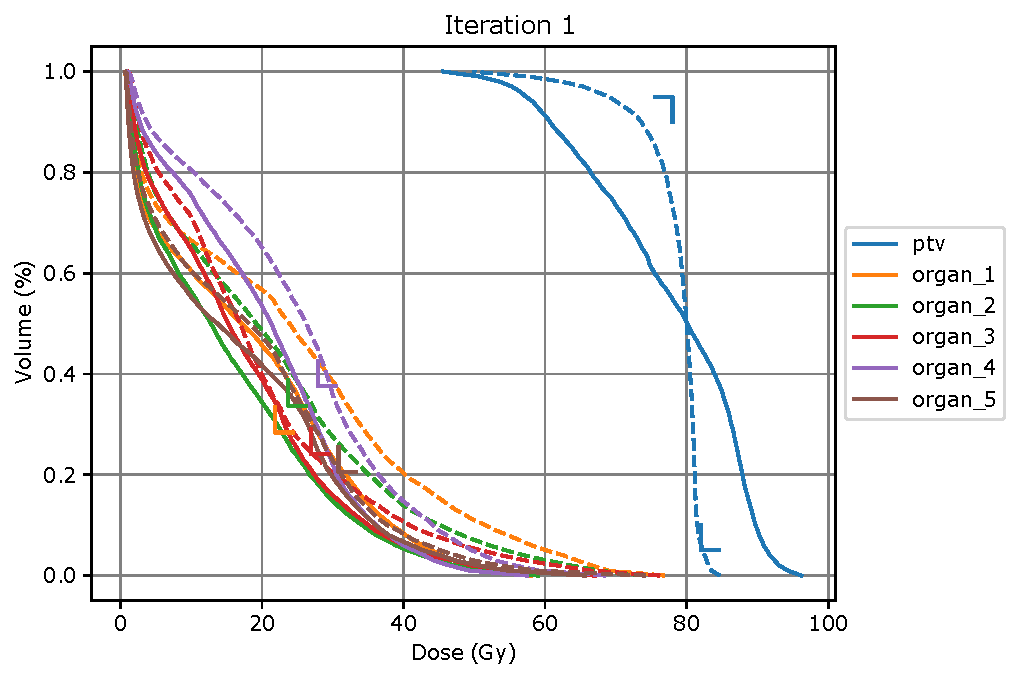
\includegraphics[width=0.49\textwidth]{AIME/distance-test-w1.pdf}	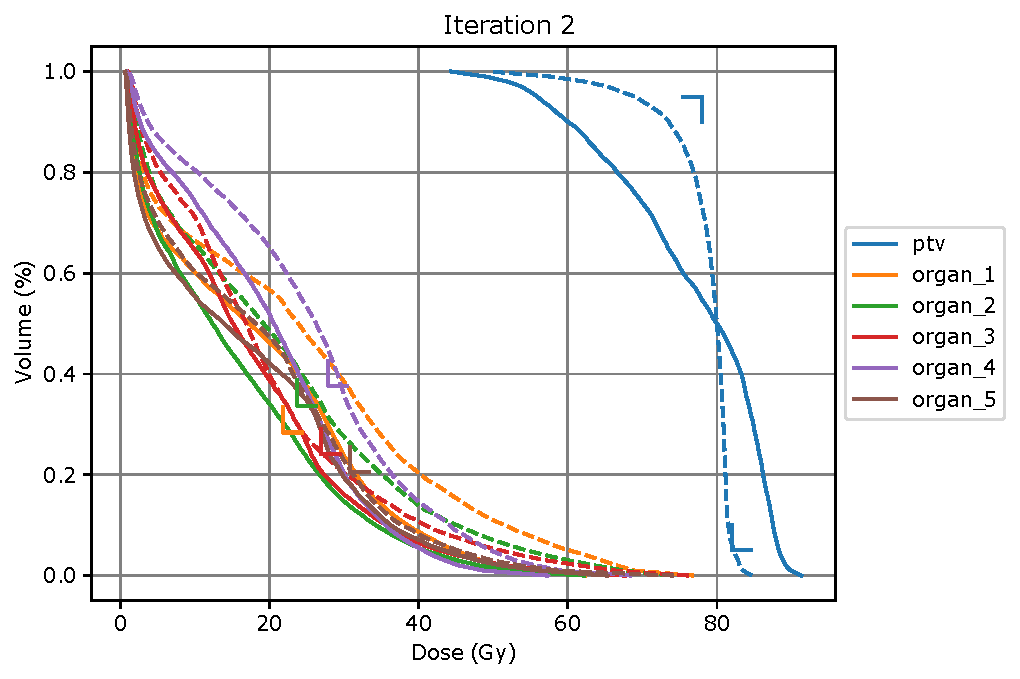
\includegraphics[width=0.49\textwidth]{AIME/distance-test-w2.pdf}	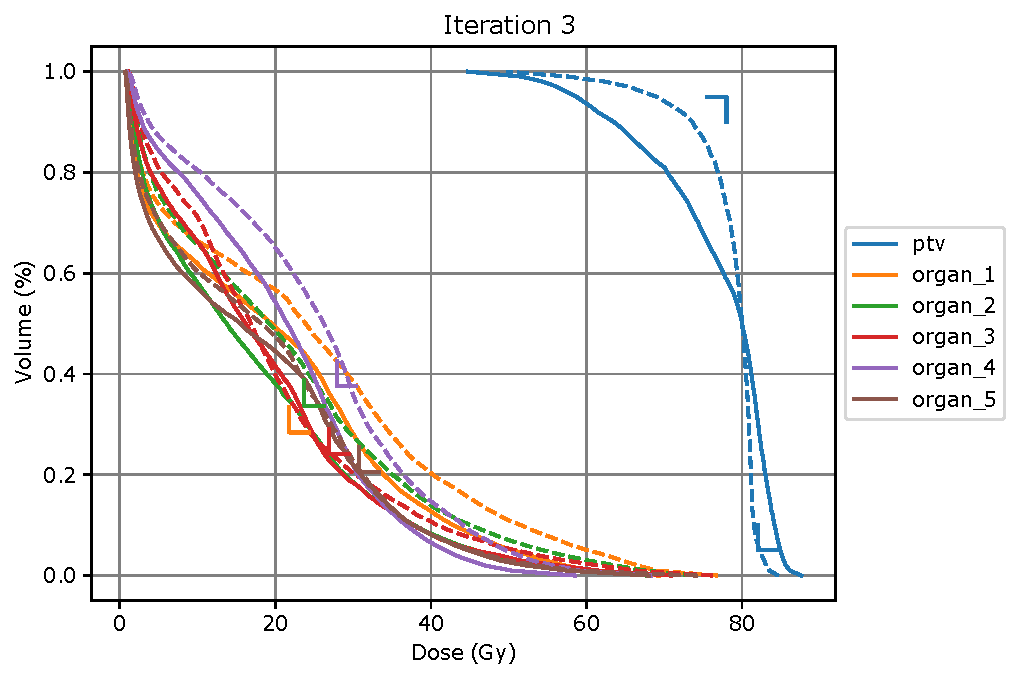
\includegraphics[width=0.49\textwidth]{AIME/distance-test-w3.pdf}	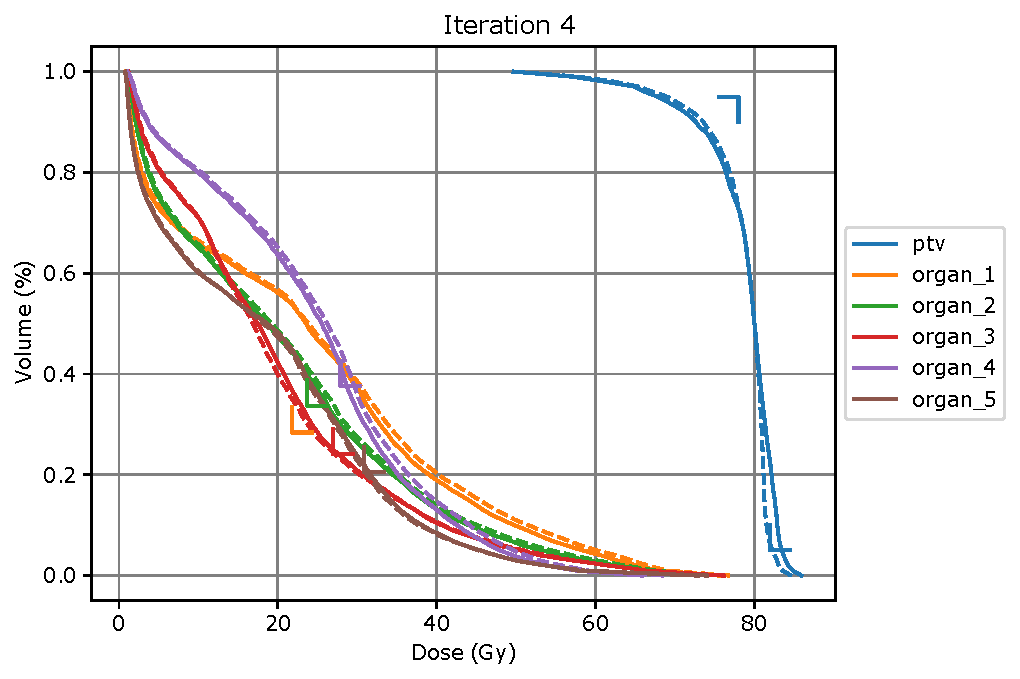
\includegraphics[width=0.49\textwidth]{AIME/distance-test-w4.pdf}
%	\caption{RL Agent DVHs after each action taken on a test (unseen) patient. Solid lines are the agent's dose DVHs; dotted ones are the reference dose DVHs (manually fine-tuned).}
%	\label{fig:steps}
%\end{figure*}

\subsection{Discussion}
%Our study demonstrates the potential of deep RL for automating radiotherapy treatment plan optimization.
%A key strength of our approach is its ability to learn from past treatment plans, capturing the complex decision-making processes of human dosimetrists.
%This data-driven approach avoids the limitations of pre-defined metrics, which may not fully capture the nuances of optimal treatment planning.
%
%However, our study also has limitations.
%The agent's performance relies on the quality and quantity of available training data.
%Cases with limited historical data or complex anatomical features may require additional strategies.
%Moreover, while the agent achieves promising results regarding dose distance reduction, the dose is not guaranteed to be clinically acceptable.
%Although this study demonstrates the promise of our RL approach in a controlled setting, one final limitation to mention is that extending it to real-world radiotherapy planning would necessitates addressing additional complexities and constraints.
%
%Several avenues exist for further research.
%Firstly, we plan to investigate strategies for incorporating additional information, such as patient characteristics and anatomical complexities, into the training process.
%Secondly, we aim to explore techniques for improving the interpretability of the agent's decision-making process, allowing for better understanding and potential clinical validation.

\subsection{Conclusion}
%Our approach differs from previous RL-based methods for radiotherapy planning in two key aspects.
%First, we avoid relying on pre-defined metrics for evaluation, which can be subjective, and limit the agent's ability to learn complex optimization strategies.
%Second, compared to traditional meta-optimization approaches, our method leverages past treatment data, potentially leading to more informed decision-making during the optimization process.
%
%This study demonstrates deep RL's feasibility and potential benefits for automating radiotherapy treatment plan optimization.
%Our approach is capable of directly predicts state evaluations, and shows promise in achieving significant improvements in efficiency and, potentially, treatment outcomes.
%Further research is needed to address limitations, improve interpretability, and ensure safe clinical integration.
%This approach could revolutionize radiotherapy planning, leading to more standardized, efficient, and improved patient care.

\subsection*{Appendix}
%As this is very new and ongoing research, we generated synthetic phantom patients and associated trustable clinical doses.
%In future work, we hope to apply this technique to real cases.

\subsubsection*{Synthetic phantom patients}
%We generated 130 patients with oval axial section bodies.
%We set the body density to water density.
%We then added an ellipsoid PTV within the body, with a slightly different density (following $\mathcal{N}(1,0.05)$).
%Likewise, we generate five organs gravitating around the PTV, aligned on the axial section.
%
%\begin{figure*}
%	\centering
%	\label{fig:main_slice-ct}
%	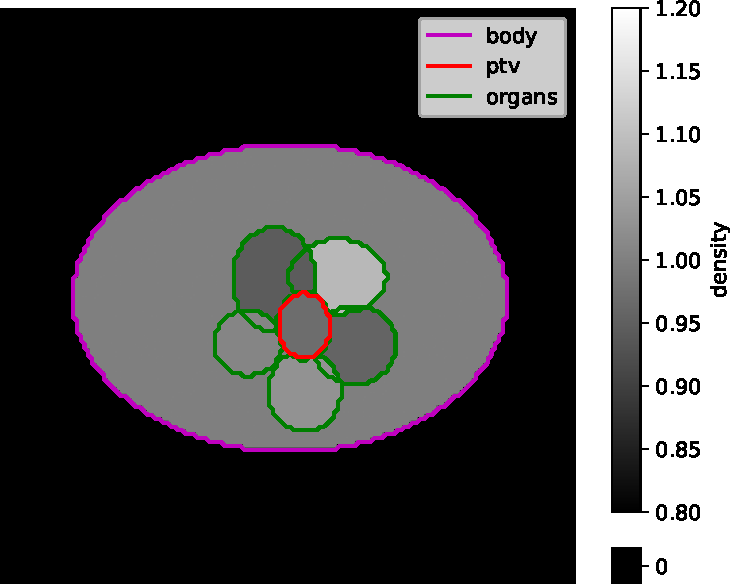
\includegraphics[height=3.5cm]{AIME/main_slice-ct.pdf}
%	\hspace{0.5cm}
%	\label{fig:main_slice-dose}
%	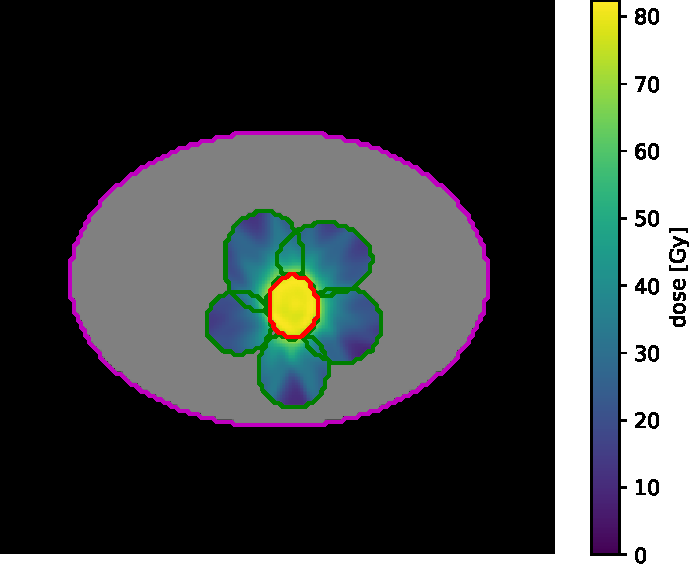
\includegraphics[height=3.5cm]{AIME/main_slice-dose.pdf}
%	%	\hspace{0.1cm}
%	\\
%	\label{fig:clinical_dvh}
%	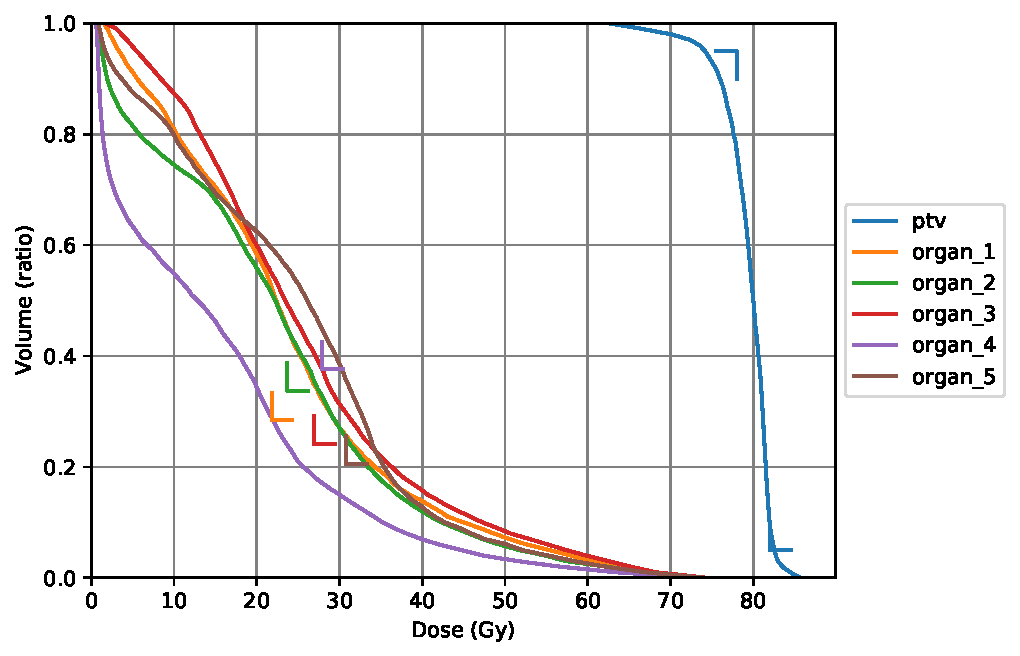
\includegraphics[width=7cm]{AIME/dvh_example.pdf}
%	\caption{
%		Example of a (generated) patient: \\
%		\textit{Left:} Main axial slice (center of the PTV) \textbf{CT}.\\
%		\textit{Right:} Main axial slice (center of the PTV) of the \textbf{clinical dose}. \\
%		\textit{Bottom:} Associated clinical dose \textbf{DVH}.
%	}
%	
%\end{figure*}
%\vspace{-1cm}

\subsubsection*{Clinical dose}
%After generating the patient's CT and structures, we needed to create a reference dose that our agent should mimic.
%We manually set weights and performed a standard optimization.
%The dose prescription is a standard 80Gy on PTV, the same across all patients.
%We used a seven-beam IMRT irradiation technique on all the cohorts.


\subsubsection*{Optimization}
%We optimize the plan using the LBFGS optimizer (shown to be the most appropriate in \cite{dubois_radiotherapy_2023}).
%For each DVH constraint (e.g. for PTV, $D_{95}>80 \ Gy$), we used a linear penalization of the overdose.



%%%%%%%%%%%%%%%%%%%%%%%%%%%%%%%%%%%%%%%%%%%%%%%%%%%%%%%%%%%%%%%%%%%%%%%%
%                                                                      %
%   %%%%%%%%%%%%%%%%%%%%%%%%%%%%%%%%%%%%%%%%%%%%%%%%%%%%%%%%%%%%%%%%   %
%   %%%%%%%%%%%%%%%%%%%%%%%%%%%%%%%%%%%%%%%%%%%%%%%%%%%%%%%%%%%%%%%%   %
%   %%%%%%%%%%%%%%%%%%%%%%%%%%%%%%%%%%%%%%%%%%%%%%%%%%%%%%%%%%%%%%%%   %
%   %%%%%%%%%%%%%%%%%%%%%%%%%%%%%%%%%%%%%%%%%%%%%%%%%%%%%%%%%%%%%%%%   %
%                                                                      %
%%%%%%%%%%%%%%%%%%%%%%%%%%%%%%%%%%%%%%%%%%%%%%%%%%%%%%%%%%%%%%%%%%%%%%%%



% Full abstract:
% https://github.com/pauldubois98/ASTRO2024/blob/main/abstract.pdf
\section{Clinically Dependent Fully Automatic Treatment Planning System (ASTRO 2024)}
\subsection{Purpose / Objective}
%Although fully automated treatment planning system (TPS) has several advantages, such as the ability to treat more patients and optimize treatments, clinics have not adopted it because there is a wide variation of practices between them.
%Additionally, dosimetrists make complex compromises while manually optimizing with a TPS, which is too complex to be captured by a metric, or not computable in a reasonable time.
%Here, we propose a solution adaptable to each clinic's practices: a reinforcement learning (RL) agent trained to mimic human dosimetrists' optimization on a cohort of previously treated patients.
%We hypothesize that by training one agent for each clinic, we ensure that guidelines specific to each of them are followed.

\subsection{Materials/Methods}
%RL agents adapt actions to situations where there are interactions with an environment.
%RL only needs a reward after performing an action.
%In the case of dose optimization, adjusting the weights of the constraints are the actions.
%The key is to find a way of rewarding the agent when making good decisions (actions) versus bad ones.
%Current RL methods in dosimetry struggle to mimic human-optimized plans.
%We propose a new reward system based on the dose distribution of past clinical cases, via calculating the DVHs differences between the agent dose, and the database dose.
%This would better guide the RL agent towards clinically-acceptable treatment plans.
%Most importantly, it also allows the optimization to fit each center's internal standard practices and guidelines.

\subsection{Results}
%We successfully trained agents to mimic the dose type of several clinics.
%We generated a cohort of 50 patients to train them and manually optimized the dose according to three guidelines.
%We then generated 20 other patients for testing purposes.
%The table shows the average difference between clinical doses and the ones optimized by our RL agents.
%Agents specializing in one type of guideline managed to mimic it, but performed poorly on others.
%Thus, for a clinically helpful, fully-automated TPS, one RL agent should be trained for each clinical guideline.

\subsection{Conclusion}
%By leveraging past clinical dose data, we have demonstrated the feasibility of training RL agents to mimic human-optimized radiotherapy plans following specific clinical guidelines.
%The results show that agents trained on specific clinic guidelines perform better in mimicking those guidelines than a single, general-purpose agent.
%This finding supports our hypothesis that a fully automatic TPS tailored to each clinic's practices is achievable.
%Future work could involve expanding the patient cohort to non-phantom cases, including modalities other than prostate cases, and real-world testing with human oversight to ensure the safety and efficacy of the RL-based TPS.
%Our research could pave the way for developing clinically-dependent automated TPS.

%Table of average DVHs distances on test cases:
%To Clinic A	To Clinic B	To Clinic C
%RL on clinic A	1.6	2.2	5.1
%RL on clinic B	2.3	1.3	2.3
%RL on clinic C	2.7	2.5	1.6
